\documentclass[aspectratio=169,xcolor=svgnames]{beamer}

\IfFileExists{preambles.tex}{\input{preambles}}{}

\usepackage{physics}
\usepackage{tikz-cd}
\usepackage{tikz}
\usepackage{xcolor}
\usepackage{mathtools}
\usepackage{dsfont}
\usepackage{amsmath}
\usepackage{ragged2e}
\usepackage[all]{xy}
\usepackage{hyperref}
\usepackage{graphicx}
\usepackage{animate}
\usepackage{xmpmulti}
\IfFileExists{movie15.sty}{\usepackage{movie15}}{}
\usepackage{multicol}
\usepackage[utf8]{inputenc}
\usepackage{algorithmic}
\usepackage{algorithm}

\usetikzlibrary{arrows.meta,positioning,shapes.geometric,calc,fit}

\setbeamertemplate{navigation symbols}{}
\setbeamersize{text margin left=0.75cm,text margin right=0.75cm}
\setbeamerfont{frametitle}{size=\large}
\setbeamerfont{block title}{size=\normalsize}
\setlength{\leftmargini}{1.1em}
\setbeamercolor{structure}{fg=DarkSlateBlue}
\setbeamercolor{block title}{bg=DarkSlateBlue,fg=white}
\setbeamercolor{block body}{bg=Lavender!45}

\newcommand{\keypoint}[1]{%
\begin{center}
\begin{beamercolorbox}[rounded=true,shadow=true,wd=0.88\textwidth,sep=0.6em,center]{block title}
#1
\end{beamercolorbox}
\end{center}
}

\newcommand{\optionalimage}[2]{%
\IfFileExists{#1}{\includegraphics[width=#2]{#1}}{%
\fbox{\parbox[c][0.24\textheight][c]{#2}{\centering Generated result image\\available in the local outputs folder}}}}

\title{Character-Conditioned Flow Matching\\for Kinetic Typography Videos}
\author[]{Xuanyu Yang}
\institute{PRIME Final Project}
\date{2026}

\begin{document}

% 1
\begingroup
\makeatletter
\ifcsname beamer@sidebarwidth\endcsname
\setlength{\hoffset}{.5\beamer@sidebarwidth}
\fi
\makeatother
\begin{frame}[plain]
\maketitle
\end{frame}
\endgroup

\section{Motivation}

% 2
\begin{frame}{Motivation: readable text in generated video}
\keypoint{Video generators can create convincing scenes while still misspelling or deforming visible text.}

\begin{itemize}
    \item A semantic prompt describes what a word means, but not its exact strokes.
    \item Character errors can flicker or accumulate across video frames.
    \item Typography in advertisements and title sequences requires both exact spelling and controlled motion.
    \item This project studies a small, interpretable alternative based on explicit visual conditions.
\end{itemize}

\[
\text{requested characters}+\text{requested motion}
\longrightarrow
\text{readable kinetic typography}
\]
\end{frame}

% 3
\begin{frame}{Why semantic tokens alone are insufficient}
\begin{columns}[T]
\column{0.48\textwidth}
\textbf{Typical text conditioning}
\[
\text{prompt}\to\text{BPE tokens}\to\text{text embedding}
\]
\begin{itemize}
    \item Good for semantic meaning
    \item Flexible natural-language input
    \item Character geometry is implicit
\end{itemize}

\column{0.48\textwidth}
\textbf{Explicit typography conditioning}
\[
\text{glyphs}+\text{positions}\to\text{visual condition}
\]
\begin{itemize}
    \item Exact requested shapes
    \item Direct spatial control
    \item Less ambiguity about spelling
\end{itemize}
\end{columns}

\keypoint{The project does not ask a semantic embedding to reconstruct letter shapes from memory.}
\end{frame}

% 4
\begin{frame}{Research question}
\begin{center}
\Large
Can a small conditional flow-matching model generate a complete video of readable, independently moving characters?
\end{center}

\vspace{0.3cm}
\begin{enumerate}
    \item Can a learned velocity field transform Gaussian video noise into typography?
    \item Do explicit glyph and position conditions preserve spelling?
    \item Does character-level conditioning outperform one rigid word-level condition?
    \item How do alignment, resolution, model width, training length, and Euler steps affect readability?
\end{enumerate}
\end{frame}

% 5
\begin{frame}{Project scope and contributions}
\begin{itemize}
    \item A synthetic English kinetic-typography dataset generated online.
    \item A pixel-space 3D U-Net trained with conditional flow matching.
    \item Whole-video generation rather than independent frame generation.
    \item Word-level and character-level glyph/position conditioning.
    \item Euler ODE sampling with optional layout guidance.
    \item Fixed-seed evaluation using MSE and thresholded glyph Dice.
    \item Reproducible training, checkpointing, GIF export, and nine core tests.
\end{itemize}

\keypoint{The contribution is a compact teaching and experimentation system, not a production text-to-video foundation model.}
\end{frame}

\section{Relation to existing approaches}

% 6
\begin{frame}{Mainstream generation versus this project}
\begin{center}
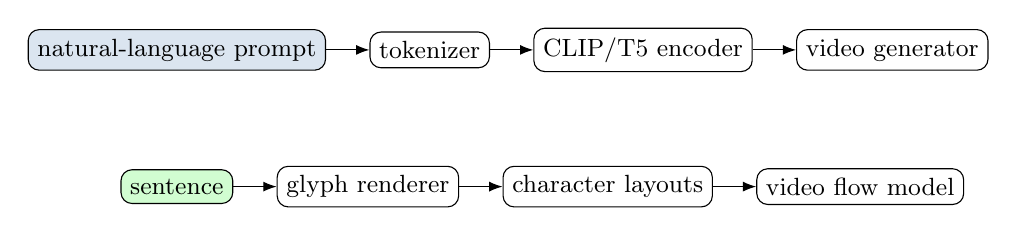
\begin{tikzpicture}[node distance=0.6cm and 0.55cm, every node/.style={font=\small}]
\node[draw,rounded corners,fill=LightSteelBlue!45] (prompt) {natural-language prompt};
\node[draw,rounded corners,right=of prompt] (tok) {tokenizer};
\node[draw,rounded corners,right=of tok] (enc) {CLIP/T5 encoder};
\node[draw,rounded corners,right=of enc] (gen) {video generator};
\draw[-{Latex}] (prompt)--(tok);
\draw[-{Latex}] (tok)--(enc);
\draw[-{Latex}] (enc)--(gen);

\node[draw,rounded corners,fill=PaleGreen!45,below=1.25cm of prompt] (sentence) {sentence};
\node[draw,rounded corners,right=of sentence] (render) {glyph renderer};
\node[draw,rounded corners,right=of render] (layout) {character layouts};
\node[draw,rounded corners,right=of layout] (flow) {video flow model};
\draw[-{Latex}] (sentence)--(render);
\draw[-{Latex}] (render)--(layout);
\draw[-{Latex}] (layout)--(flow);
\end{tikzpicture}
\end{center}

\begin{itemize}
    \item The current project has no learned language tokenizer or semantic text encoder.
    \item Whitespace splitting only schedules which word appears during each frame segment.
    \item The model receives rasterized visual shapes rather than token IDs.
\end{itemize}
\end{frame}

% 7
\begin{frame}{Relationship to TextDiffuser}
\begin{itemize}
    \item TextDiffuser adds explicit character-level segmentation masks and layout guidance to image diffusion.
    \item TextDiffuser-2 combines ordinary prompt BPE tokens with character tokens and coordinate tokens.
    \item Those systems generate styled images and backgrounds at large scale.
    \item This project follows the same broad principle of explicit text geometry, but applies it to a small video flow model.
\end{itemize}

\vspace{0.15cm}
\begin{center}
\begin{tabular}{lcc}
\hline
 & TextDiffuser family & This project \\
\hline
Output & image & short video tensor \\
Generator & diffusion & flow matching \\
Text condition & tokens/masks/boxes & glyphs/heatmaps \\
Spatial unit & line or character & character per frame \\
\hline
\end{tabular}
\end{center}
\end{frame}

\section{Synthetic data and conditions}

% 8
\begin{frame}{Synthetic training dataset}
\begin{itemize}
    \item Training examples are rendered online with Pillow; no video download is required.
    \item Short English sentences are sampled from verbs, nouns, adjectives, and templates.
    \item Example scripts:
    \[
    \texttt{MAKE TEXT MOVE},\quad
    \texttt{CREATE THE FUTURE},\quad
    \texttt{STAY CURIOUS}.
    \]
    \item Motion families: horizontal, vertical, bounce, and circle.
    \item Current character model: 12 grayscale frames at $64\times128$ resolution.
    \item Rendering is deterministic for a given dataset index and seed.
\end{itemize}

\keypoint{Synthetic data provides exact ground-truth spelling, layout, and trajectory for every frame.}
\end{frame}

% 9
\begin{frame}{A sentence becomes a video timeline}
For a 12-frame, three-word sentence:
\[
\underbrace{0,1,2,3}_{\texttt{MAKE}}
\quad
\underbrace{4,5,6,7}_{\texttt{TEXT}}
\quad
\underbrace{8,9,10,11}_{\texttt{MOVE}}.
\]

\begin{center}
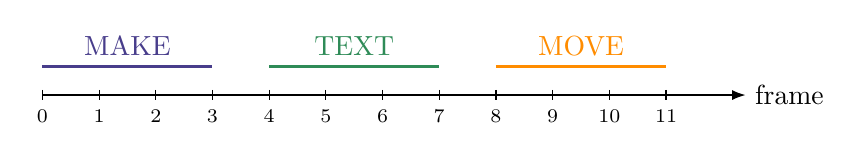
\begin{tikzpicture}[x=0.72cm,y=0.8cm]
\draw[-{Latex}] (0,0)--(12.4,0) node[right]{frame};
\foreach \x in {0,...,11}{\draw (\x,0.08)--(\x,-0.08) node[below]{\scriptsize \x};}
\draw[very thick,DarkSlateBlue] (0,0.45)--(3,0.45) node[midway,above]{MAKE};
\draw[very thick,SeaGreen] (4,0.45)--(7,0.45) node[midway,above]{TEXT};
\draw[very thick,DarkOrange] (8,0.45)--(11,0.45) node[midway,above]{MOVE};
\end{tikzpicture}
\end{center}

\begin{itemize}
    \item The entire timeline is one model output.
    \item Word changes are planned explicitly; the model is not performing language generation.
\end{itemize}
\end{frame}

% 10
\begin{frame}{From word-level to character-level motion}
\begin{columns}[T]
\column{0.47\textwidth}
\textbf{Word-level baseline}
\[
\texttt{MAKE}\to(g_{\text{word}},p_{\text{word}}(t))
\]
All letters move as one rigid raster object.

\column{0.47\textwidth}
\textbf{Character-level model}
\[
\begin{aligned}
M&\to(g_1,p_1(t)),\\
A&\to(g_2,p_2(t)),\\
K&\to(g_3,p_3(t)),\\
E&\to(g_4,p_4(t)).
\end{aligned}
\]
Each letter has an independent condition and trajectory.
\end{columns}

\keypoint{Character-level control directly implements the requested ``character shape + character position'' idea.}
\end{frame}

% 11
\begin{frame}{Per-character condition tensor}
The model supports at most $K=8$ characters per displayed word.

\begin{center}
\begin{tabular}{lll}
\hline
Condition & Shape & Meaning \\
\hline
Canonical glyphs & $K\times T\times H\times W$ & one centered glyph per channel \\
Position maps & $K\times T\times H\times W$ & one Gaussian heatmap per character \\
Aligned layouts & $K\times T\times H\times W$ & glyph translated to its requested center \\
Target video & $1\times T\times H\times W$ & composite typography frames \\
\hline
\end{tabular}
\end{center}

\[
8\ \text{glyph}+8\ \text{position}+8\ \text{layout}
=24\ \text{condition channels}.
\]

Unused character slots are padded with zeros.
\end{frame}

% 12
\begin{frame}{Independent character trajectories}
The word follows a base trajectory $(x_{\mathrm{base}}(t),y_{\mathrm{base}}(t))$.
Character $i$ receives a phase-shifted vertical offset:
\[
y_i(t)=y_{\mathrm{base}}(t)
+A\sin\left(\frac{2\pi t}{T}+\frac{i\pi}{3}\right).
\]

Horizontal positions preserve readable word spacing:
\[
x_i(t)=x_{\mathrm{base}}(t)-\frac{W_{\mathrm{word}}}{2}
+\sum_{j<i}(w_j+s)+\frac{w_i}{2}.
\]

\begin{itemize}
    \item Every character has a distinct coordinate at every frame.
    \item The letters move independently without losing their order.
    \item Each coordinate is converted into a Gaussian heatmap.
\end{itemize}
\end{frame}

\section{Conditional flow matching}

% 13
\begin{frame}{Source and data distributions}
Let a complete video be a high-dimensional tensor:
\[
x\in\mathbb{R}^{C\times T\times H\times W}.
\]

Define:
\[
x_0\sim\mathcal{N}(0,I)
\qquad\text{and}\qquad
x_1\sim q_{\mathrm{data}}(x\mid g,p,\ell),
\]
where $g$ is glyph shape, $p$ is position, and $\ell$ is aligned layout.

\begin{center}
\[
\text{Gaussian noise video}
\xrightarrow{\text{learned continuous flow}}
\text{kinetic typography video}
\]
\end{center}

\keypoint{Noise and target have the same full-video shape; generation is not frame-by-frame.}
\end{frame}

% 14
\begin{frame}{Conditional probability path}
Choose the straight interpolation:
\[
x_t=(1-t)x_0+t x_1,
\qquad t\sim\mathcal{U}(0,1).
\]

\begin{itemize}
    \item $t=0$: a complete Gaussian-noise clip.
    \item $t=1$: a complete clean typography clip.
    \item Intermediate $t$: every frame is partially corrupted.
\end{itemize}

\begin{center}
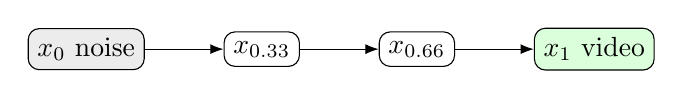
\begin{tikzpicture}[node distance=1.0cm]
\node[draw,rounded corners,fill=Gray!15] (a) {$x_0$ noise};
\node[draw,rounded corners,right=of a] (b) {$x_{0.33}$};
\node[draw,rounded corners,right=of b] (c) {$x_{0.66}$};
\node[draw,rounded corners,fill=PaleGreen!35,right=of c] (d) {$x_1$ video};
\draw[-{Latex}] (a)--(b);
\draw[-{Latex}] (b)--(c);
\draw[-{Latex}] (c)--(d);
\end{tikzpicture}
\end{center}
\end{frame}

% 15
\begin{frame}{Target conditional velocity}
Differentiate the straight path:
\[
\frac{d x_t}{dt}=x_1-x_0.
\]

The supervised target is therefore:
\[
u_t(x_t\mid x_0,x_1)=x_1-x_0.
\]

The neural vector field predicts:
\[
v_\theta(x_t,t,g,p,\ell).
\]

\begin{itemize}
    \item Gaussian noise $x_0$, clean video $x_1$, and time $t$ are sampled for every batch.
    \item The exact conditional velocity can be calculated without simulating an ODE during training.
\end{itemize}
\end{frame}

% 16
\begin{frame}{Conditional flow-matching objective}
The basic loss is:
\[
\mathcal{L}_{\mathrm{CFM}}
=
\mathbb{E}
\left[
\left\|
v_\theta(x_t,t,g,p,\ell)-(x_1-x_0)
\right\|_2^2
\right].
\]

For each training batch:
\begin{enumerate}
    \item render sentence video and all character conditions;
    \item sample Gaussian video $x_0$;
    \item sample $t\sim\mathcal{U}(0,1)$;
    \item construct $x_t$;
    \item regress the velocity $x_1-x_0$.
\end{enumerate}

\keypoint{Training requires one network evaluation; numerical integration is only used for generation.}
\end{frame}

% 17
\begin{frame}{Foreground-weighted velocity loss}
Most video pixels are black background, so ordinary MSE can underweight thin strokes.

Define a soft foreground mask:
\[
m=\mathrm{clip}\left(\frac{x_1+1}{2},0,1\right),
\qquad
w=1+\lambda_{\mathrm{fg}}m.
\]

The project uses:
\[
\mathcal{L}_{\mathrm{weighted}}
=
\frac{\mathbb{E}[w\,\|v_\theta-u_t\|^2]}{\mathbb{E}[w]},
\qquad \lambda_{\mathrm{fg}}=5.
\]

\begin{itemize}
    \item Background pixels still contribute to the loss.
    \item Character strokes receive additional weight.
    \item This increased predicted foreground intensity and reduced faded letters.
\end{itemize}
\end{frame}

\section{Model and sampling}

% 18
\begin{frame}{Compact 3D U-Net vector field}
\begin{center}
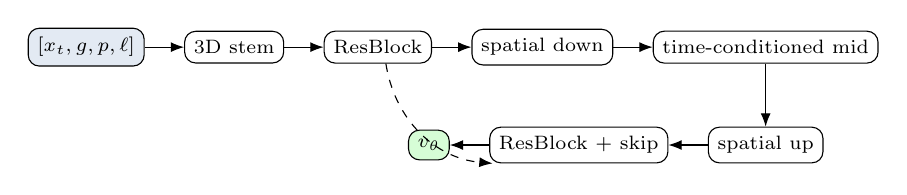
\begin{tikzpicture}[node distance=0.55cm and 0.5cm,every node/.style={font=\scriptsize}]
\node[draw,rounded corners,fill=LightSteelBlue!35] (in) {$[x_t,g,p,\ell]$};
\node[draw,rounded corners,right=of in] (stem) {3D stem};
\node[draw,rounded corners,right=of stem] (enc) {ResBlock};
\node[draw,rounded corners,right=of enc] (down) {spatial down};
\node[draw,rounded corners,right=of down] (mid) {time-conditioned mid};
\node[draw,rounded corners,below=0.8cm of mid] (up) {spatial up};
\node[draw,rounded corners,left=of up] (dec) {ResBlock + skip};
\node[draw,rounded corners,fill=PaleGreen!40,left=of dec] (out) {$v_\theta$};
\draw[-{Latex}] (in)--(stem);
\draw[-{Latex}] (stem)--(enc);
\draw[-{Latex}] (enc)--(down);
\draw[-{Latex}] (down)--(mid);
\draw[-{Latex}] (mid)--(up);
\draw[-{Latex}] (up)--(dec);
\draw[-{Latex}] (dec)--(out);
\draw[-{Latex},dashed] (enc) to[bend right=38] (dec);
\end{tikzpicture}
\end{center}

\begin{itemize}
    \item 3D convolutions observe neighboring pixels and neighboring frames.
    \item Spatial dimensions are compressed; the temporal length is preserved.
    \item The selected model uses 16 base channels and about 0.62M parameters.
\end{itemize}
\end{frame}

% 19
\begin{frame}{Continuous-time conditioning and temporal consistency}
The scalar time is embedded by an MLP:
\[
e_t=\mathrm{MLP}(t).
\]
Each residual block uses FiLM modulation:
\[
h'=\mathrm{Norm}(h)\odot(1+s(e_t))+b(e_t).
\]

\begin{itemize}
    \item The same network predicts velocities at every continuous flow time.
    \item 3D kernels couple adjacent frames and reduce independent frame flicker.
    \item The model predicts a velocity tensor with exactly the video shape.
\end{itemize}

\keypoint{Time in the ODE and time inside the video are different axes: flow time transforms the complete temporal clip.}
\end{frame}

% 20
\begin{frame}{Training pipeline}
\begin{center}
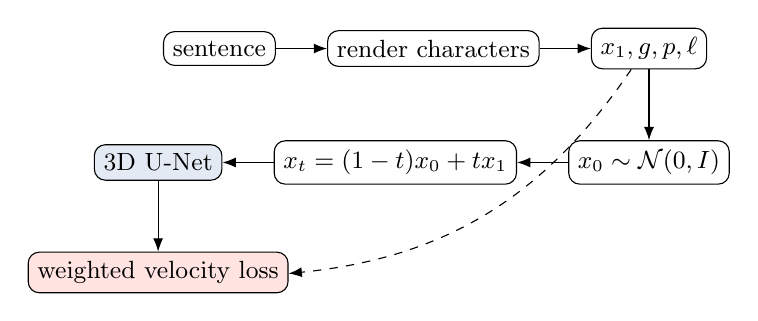
\begin{tikzpicture}[node distance=0.65cm and 0.65cm,every node/.style={font=\small}]
\node[draw,rounded corners] (text) {sentence};
\node[draw,rounded corners,right=of text] (data) {render characters};
\node[draw,rounded corners,right=of data] (target) {$x_1,g,p,\ell$};
\node[draw,rounded corners,below=0.9cm of target] (noise) {$x_0\sim\mathcal N(0,I)$};
\node[draw,rounded corners,left=of noise] (mix) {$x_t=(1-t)x_0+t x_1$};
\node[draw,rounded corners,left=of mix,fill=LightSteelBlue!35] (net) {3D U-Net};
\node[draw,rounded corners,below=0.9cm of net,fill=MistyRose] (loss) {weighted velocity loss};
\draw[-{Latex}] (text)--(data);
\draw[-{Latex}] (data)--(target);
\draw[-{Latex}] (target)--(noise);
\draw[-{Latex}] (noise)--(mix);
\draw[-{Latex}] (mix)--(net);
\draw[-{Latex}] (net)--(loss);
\draw[-{Latex},dashed] (target) to[bend left=25] (loss);
\end{tikzpicture}
\end{center}

\begin{itemize}
    \item Optimizer: AdamW, learning rate $2\times10^{-4}$.
    \item Mixed precision, gradient clipping, CSV logging, and resumable checkpoints.
\end{itemize}
\end{frame}

% 21
\begin{frame}{Euler ODE sampling}
After training, solve:
\[
\frac{d x_t}{dt}=v_\theta(x_t,t,g,p,\ell).
\]

With $N$ steps and $h=1/N$:
\[
x_{k+1}=x_k+h\,v_\theta\left(x_k,\frac{k}{N},g,p,\ell\right).
\]

\begin{enumerate}
    \item sample one complete Gaussian video;
    \item predict the conditional velocity;
    \item take one Euler step;
    \item repeat until $t=1$;
    \item threshold the grayscale mask and export an aspect-preserving GIF.
\end{enumerate}

For crisp binary typography, validation selected $N=20$ and threshold $-0.5$.
\end{frame}

% 22
\begin{frame}{Aligned layout and optional sampling guidance}
Canonical glyphs begin at the center of the canvas. Aligned layouts translate them to their requested character coordinates.

An optional guided velocity is:
\[
v_{\mathrm{guided}}
=v_\theta
+s\frac{\ell-x_t}{1-t}.
\]

\begin{itemize}
    \item Word-level validation benefited slightly from $s=0.1$.
    \item Strong guidance damaged strokes because of subpixel alignment error.
    \item The final character model is accurate enough without additional guidance.
\end{itemize}

\keypoint{Alignment was more important than simply training longer or increasing model width.}
\end{frame}

\section{Experiments}

% 23
\begin{frame}{Experimental protocol}
\begin{columns}[T]
\column{0.49\textwidth}
\textbf{Training}
\begin{itemize}
    \item RTX 5070, 12 GB
    \item 12 frames, $64\times128$
    \item batch size 4
    \item base channels 16
    \item 10,000 steps
    \item maximum 8 characters
\end{itemize}

\column{0.49\textwidth}
\textbf{Fixed validation}
\begin{itemize}
    \item 8 synthetic sentences
    \item data seed 9000
    \item noise seed 123
    \item 20 Euler steps
    \item MSE and mask Dice
    \item threshold sweep
\end{itemize}
\end{columns}

\[
\mathrm{Dice}=\frac{2|M_{\mathrm{target}}\cap M_{\mathrm{generated}}|}
{|M_{\mathrm{target}}|+|M_{\mathrm{generated}}|}.
\]
\end{frame}

% 24
\begin{frame}{Development progression}
\begin{center}
\begin{tabular}{p{2.2cm}p{3.2cm}p{5.6cm}}
\hline
Stage & Change & Observation \\
\hline
Smoke test & $32\times32$ words & Pipeline worked; quality was not meaningful. \\
Sentence model & word changes over time & Learned sequences, but unseen words were weak. \\
Aligned word & glyph moved to target position & Major readability and convergence improvement. \\
Weighted loss & emphasize sparse strokes & Foreground became stronger. \\
$64\times128$ & larger native glyphs & Best word-level resolution. \\
Character model & 24 explicit condition channels & Independent motion and near-perfect mask accuracy. \\
\hline
\end{tabular}
\end{center}

\keypoint{Each failed or weaker stage identified a concrete limitation in representation, loss, or spatial alignment.}
\end{frame}

% 25
\begin{frame}{Alignment and training-length ablations}
\begin{center}
\begin{tabular}{lcc}
\hline
Word-level setting & MSE $\downarrow$ & Dice $\uparrow$ \\
\hline
$48\times96$, weighted & 0.0202 & 0.7460 \\
$64\times128$, 10k & 0.01015 & 0.77754 \\
$64\times128$, 20k & 0.01131 & 0.77110 \\
$64\times128$, 10k + guidance 0.1 & 0.00915 & 0.78585 \\
\hline
\end{tabular}
\end{center}

\begin{itemize}
    \item Continuing from 10k to 20k slightly reduced validation quality.
    \item Fixed-seed evaluation selected the 10k checkpoint by early stopping.
    \item Small layout guidance improved Dice; strong guidance did not.
\end{itemize}
\end{frame}

% 26
\begin{frame}{Resolution, model width, and Euler steps}
\begin{columns}[T]
\column{0.5\textwidth}
\textbf{Architecture ablations}
\begin{center}
\begin{tabular}{lc}
\hline
Setting & Dice \\
\hline
$64\times128$, base 16 & 0.7775 \\
$64\times128$, base 24 & 0.7548 \\
$96\times192$, base 16 & 0.7616 \\
\hline
\end{tabular}
\end{center}

\column{0.5\textwidth}
\textbf{Euler-step ablation}
\begin{center}
\begin{tabular}{lc}
\hline
Steps & Dice \\
\hline
20 & 0.78585 \\
40 & 0.78433 \\
60 & 0.78279 \\
100 & 0.78125 \\
\hline
\end{tabular}
\end{center}
\end{columns}

\keypoint{More pixels, more channels, more training, or more ODE steps did not automatically improve readable masks.}
\end{frame}

% 27
\begin{frame}{Character-level quantitative results}
\begin{center}
\begin{tabular}{lcc}
\hline
Checkpoint & MSE $\downarrow$ & Dice at $-0.5$ $\uparrow$ \\
\hline
3,000 steps & 0.000120 & 0.990236 \\
5,000 steps & 0.000114 & 0.995504 \\
10,000 steps & \textbf{0.000017} & \textbf{0.995737} \\
\hline
Word-level best & 0.009147 & 0.785849 \\
\hline
\end{tabular}
\end{center}

\begin{itemize}
    \item The 10k character checkpoint is selected as \texttt{model\_best.pt}.
    \item Separate aligned character layouts make the conditional task substantially easier.
    \item The large improvement should not be attributed only to network architecture; the condition is also more informative.
\end{itemize}
\end{frame}

% 28
\begin{frame}{Qualitative character motion}
\begin{columns}[T]
\column{0.56\textwidth}
\begin{center}
\optionalimage{outputs/english_character_128/contact_sheet.png}{0.98\linewidth}
\end{center}

\column{0.41\textwidth}
\begin{itemize}
    \item Each letter moves with its own vertical phase.
    \item Character order and word readability are preserved.
    \item Examples include:
    \begin{itemize}
        \item MAKE $\to$ TEXT $\to$ MOVE
        \item HELLO $\to$ NEW $\to$ WORLD
        \item CREATE $\to$ YOUR $\to$ STORY
    \end{itemize}
    \item GIF files are stored under \texttt{outputs/english\_character\_128/}.
\end{itemize}
\end{columns}
\end{frame}

\section{Limitations and conclusion}

% 29
\begin{frame}{Limitations and next steps}
\begin{itemize}
    \item The renderer currently uses uppercase grayscale glyphs on a black background.
    \item A displayed word is limited to eight characters in the current checkpoint.
    \item Sentence timing is predefined rather than inferred from natural language.
    \item Explicit aligned layouts make spelling easy but reduce the amount of visual structure the model must invent.
    \item Motion is generated from four procedural trajectory families.
    \item Thresholded masks are crisp, but this is not yet advertising-quality styled typography.
\end{itemize}

\vspace{0.15cm}
\textbf{Next extension:} add a per-character color schedule
\[
C\in\mathbb{R}^{K\times T\times3},
\]
then map user descriptions such as ``rainbow letters'' into character-level RGB conditions.
\end{frame}

% 30
\begin{frame}{Conclusion}
\keypoint{Explicit character geometry and position turned a blurry word-level prototype into a controllable kinetic-typography flow model.}

\begin{itemize}
    \item A complete video is generated by transporting Gaussian noise through a learned ODE.
    \item The model conditions on separate glyph, position, and aligned-layout channels for every character.
    \item 3D convolutions model spatial structure and temporal consistency jointly.
    \item Fixed validation selected a 10k character model with Dice $0.995737$.
    \item The project demonstrates why explicit visual text information is complementary to semantic token embeddings.
\end{itemize}

\vspace{0.2cm}
\begin{center}
\Large
Noise $\longrightarrow$ learned velocity field $\longrightarrow$ readable moving characters
\end{center}
\end{frame}

\end{document}
